\documentclass{article}
\usepackage[utf8]{inputenc}
\usepackage{mathtools, amssymb, amsthm}
\usepackage{fullpage}
\usepackage{physics}
\usepackage{siunitx}
\usepackage{comment}

\usepackage{tikz}
\usetikzlibrary{arrows}

\usepackage[
    pdfusetitle,
    colorlinks
]{hyperref}

\title{Modeling and simulation of the SLM process}
\date{\today}
\author{Oleg Rogozin}

\newcommand{\dder}[2][]{\Delta_{#2}#1}
\newcommand{\diag}[1]{\qty(#1)^\mathrm{diag}}
\newcommand{\fusion}[1]{{#1}^\mathrm{fus}}

% dimensionless variables
\newcommand{\Hx}{\hat{x}}
\newcommand{\Ht}{\hat{t}}
\newcommand{\Hh}{\hat{h}}
\newcommand{\HT}{\hat{T}}
\newcommand{\HP}{\hat{P}}
\newcommand{\Halpha}{\hat{\alpha}}
\newcommand{\Hsigma}{\hat{\sigma}}
\newcommand{\Hf}{\hat{f}}
\newcommand{\Hc}{\hat{c}}
\newcommand{\Hk}{\hat{k}}
\newcommand{\Hphi}{\hat{\phi}}
\newcommand{\Hpsi}{\hat{\psi}}
\newcommand{\HR}{\hat{R}}

\begin{document}
\maketitle
\tableofcontents

\section{Formulation of the problem}

%%% The first law of thermodynamics
The conservation of energy for a substance at rest is described by the \(D\)-dimensional heat-conduction equation
\begin{equation}\label{eq:heat_conduction}
	\rho\pdv{h(T)}{t} = \pdv{x_i}\qty( k(\psi,T)\pdv{T}{x_i} ),
\end{equation}
where \(x_i\) are the physical coordinates (\si{m}), \(t\) is the time (\si{s}),
\(\rho\) is the density (\si{kg/m}\(^D\)), \(h\) is the specific enthalpy (\si{J/kg}),
\(T\) is the temperature (\si{\K}), \(k\) is the thermal conductivity (\si{W/Km}\(^{D-2}\)),
\(\psi\) is the porosity. Let
\begin{equation}\label{eq:porosity_variables}
	\rho = \rho_0(1-\psi_0), \quad k = k_0(T)(1-\psi),
\end{equation}
where \(\rho_0\) and \(k_0\) is the density and thermal conductivity of the bulk material, respectively,
\(\psi_0\) is the initial porosity.

%%% Introduce a liquid fraction
To incorporate the fusion process into the model, let the enthalpy depends on the temperature as follows:
\begin{equation}\label{eq:enthalpy}
	h = \int_{T_0}^T c_p(\xi)\dd{\xi} + \fusion{h}\phi(h),
\end{equation}
where \(c_p\) is the specific heat capacity (\si{J/kgK}), \(\fusion{h}\) is the specific enthalpy of fusion (\si{J/kg}),
\(\phi\) is the liquid fraction (\(0 \leq \phi \leq 1\)).
\(\phi=0\) and \(\phi=1\) corresponds to the solid and liquid states, respectively.
Substituting~\eqref{eq:porosity_variables} and~\eqref{eq:enthalpy} into~\eqref{eq:heat_conduction}, we obtain
\begin{equation}\label{eq:heat_conduction2}
	\rho_0\pdv{h}{t} = \pdv{x_i}\qty( \frac{1-\psi}{1-\psi_0} \frac{k_0(T)}{c_p(T)}\pdv{h_*}{x_i} ),
\end{equation}
where \(h_* = h - \fusion{h}\phi\) is introduced for convenience.

%%% Change in thermophysical properties resulting from fusion process
The phase transition results in an abrupt change in the thermophysical properties \(f=c_p,k_0\) of the material;
therefore, they can be expressed as
\begin{equation}\label{eq:fusion_change}
	f = f_S(T) + \qty( f_L(T) - f_S(T) )\phi,
\end{equation}
where \(f_S\) and \(f_L\) correspond to solid and liquid properties.
The porosity change is irreversible in time:
\begin{equation}\label{eq:porosity}
	\psi(t) = \psi_0\min_{0\leq\tau\leq t}\qty( 1-\phi(h(\tau)) ).
\end{equation}

%%% Initial and boundary conditions
Consider a half-space problem \(x_D<0\) with the following boundary condition at \(x_D=0\):
\begin{equation}\label{eq:bc}
	k(\psi,T)\pdv{T}{x_D} = \frac{A(\psi)P}{(\pi R^2)^{(D-1)/2}}\exp\qty( -\frac{(x_i-x_{Bi}(t))^2}{R^2} )
	    - \alpha(T-T_0) - \epsilon\sigma T^{D+1},
\end{equation}
where \(A\) is the absorptivity, \(P\) is the laser power (\si{W}), \(R\) is the radius of the laser beam (\si{m}),
\(x_{Bi}\) are the coordinates of its center (\si{m}), \(\alpha\) is the convective heat transfer coefficient (\si{W/Km}\(^{D-1}\)),
\(\epsilon\) is the emissivity, \(\sigma\) is the Stefan--Boltzmann constant (\si{W/K}\(^{D+1}\)\si{m}\(^{D-1}\)).
The initial condition is \(T=T_0\) at \(t=0\).

\subsection{Dimensionless expressions}

Introduce the following dimensionless variables:
\begin{equation}\label{eq:dimensionless}
    \begin{aligned}
        x_i &= \Hx_iR, & t &= \Ht t_0, & h &= \Hh c_p(T_0)\Delta{T}, & T - T_0 &= \HT\Delta{T}, \\
        P &= \HP k_0(T_0)\Delta{T}R^{D-2}, & \alpha &= \Halpha\frac{k_0(T_0)}R, &
            \sigma &= \Hsigma\frac{k_0(T_0)}{R\Delta{T}^D}, & T_0 &= \HT_0\Delta{T}, \\
    \end{aligned}
\end{equation}
where \(t_0 = \rho_0 c_p(T_0) R^2/k_0(T_0)\) is the diffusive time scale at \(T=T_0\),
\(\Delta{T} = (T_S+T_L)/2 - T_0\) is the unit temperature,
\(T_S\) and \(T_L\) are the solidus and liquidus temperatures, respectively.
If \(|\pdv*{x_{Bi}}{t}|\) is of order \(U_0\), where \(U_0\) is the reference scanning speed (\si{m/s}),
then \(R/U_0\) is the convective time scale. Also denote
\begin{equation}\label{eq:dimensionless2}
    \Hc_p(\HT) = \frac{c_p(T)}{c_p(T_0)}, \quad
    \Hk_0(\HT) = \frac{k_0(T)}{k_0(T_0)}, \quad
    \Hphi(\Hh) = \phi(h), \quad
    \Hpsi(\Hh) = \psi(h).
\end{equation}
Then~\eqref{eq:enthalpy},~\eqref{eq:heat_conduction2}, and~\eqref{eq:bc} take the following nondimensional form:
\begin{gather}
	\Hh_* \equiv \Hh - \fusion{\Hh}\Hphi = \int_0^{\HT} \Hc_p(\xi)\dd{\xi}, \label{eq:enthalpy_hats} \\
	\pdv{\Hh}{\Ht} = \pdv{\Hx_i}\qty(
	    \frac{1-\Hpsi}{1-\psi_0}
	    \frac{\Hk_0(\HT)}{\Hc_p(\HT)}\pdv{\Hh_*}{\Hx_i}
	), \label{eq:heat_conduction_hats} \\
	\qty(1 - \Hpsi) \frac{\Hk_0(\HT)}{\Hc_p(\HT)}\pdv{\Hh_*}{\Hx_D} +
	    \Halpha\HT + \epsilon\Hsigma \qty(\HT + \HT_0)^{D+1} =
	    \frac{A(\Hpsi)\HP}{\pi^{(D-1)/2}}\exp\qty( -\qty(\Hx_i-\Hx_{Bi}(t))^2 ). \label{eq:bc_hats}
\end{gather}
The initial condition is \(\Hh = 0\).

\subsection{Thermophysical properties}

For conventional materials, the required thermophysical properties can be reasonably approximated
by the three-parameter model (Fig.~\ref{fig:thermophysical})
\begin{equation}\label{eq:thermophysical_model}
	\Hf = 1 + \Hf'_S\HT + \qty[
	    \fusion{\Hf} + \qty(\Hf'_L-\Hf'_S) \qty(\HT-1)
	]\Hphi,
\end{equation}
where \(\Hf'_{S,L}\) are the corresponding constant first temperature derivatives far from fusion process,
\(\fusion{\Hf}\) is the property jump at the phase transition.
Matching~\eqref{eq:thermophysical_model} with~\eqref{eq:fusion_change}, we obtain
\begin{equation}\label{eq:thermophysical_model_explicit}
	\Hf_S = 1 + \Hf'_S\HT, \quad
	\Hf_L = \Hf_{L0} + \Hf'_L\HT,
\end{equation}
where \(\Hf_{L0} = 1 + \Hf'_S - \Hf'_L + \fusion{\Hf}\).

\begin{figure}
    \centering
    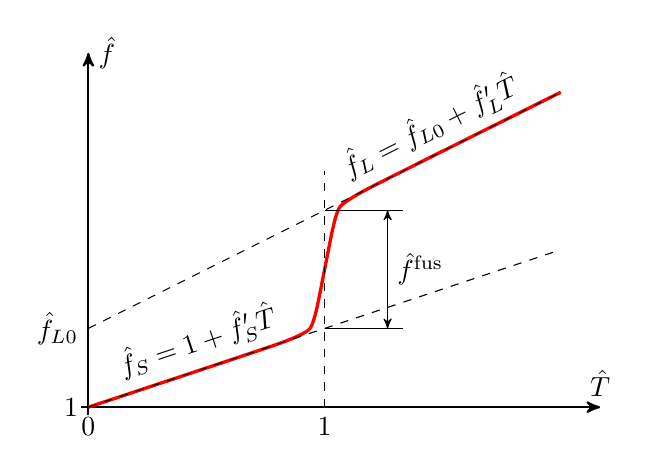
\begin{tikzpicture}[thick, >=stealth']
        \coordinate (O) at (0,0);
        \draw[->] (-0.1,0) -- (6.5,0) node[above] {$\HT$};
        \draw[->] (0,-0.1) -- (0,4.5) node[right] {$\Hf$};

        \path (O) -- (3,1) node[midway,sloped,above] {$\Hf_S=1+\Hf'_S\HT$}
            -- (3,2.5) -- (6,4) node[midway,sloped,above] {$\Hf_L=\Hf_{L0}+\Hf'_L\HT$};
        \draw[red, very thick] plot[smooth,tension=0.3,mark=] coordinates{
            (0,0) (2.4,2.4/3) (2.8, 2.8/3+0.05) (2.9,3.5/2-0.5) (3.1,3.5/2+0.5) (3.2,2.5+0.2/2-0.05) (3.6,2.5+0.6/2) (6,4)};
        \draw[thin,dashed] (0,1) coordinate(A) -- (6,4);
        \draw[thin,dashed] (O) -- (6,2);
        \draw[thin,dashed] (3,0) coordinate(F) -- (3,3);

        \node[below] at (O) {$0$};
        \node[below] at (F) {$1$};
        \node[left] at (O) {$1$};
        \node[left] at (A) {$\Hf_{L0}$};

        \draw[thin] (3,1) -- (4,1);
        \draw[thin] (3,2.5) -- (4,2.5);
        \draw[thin,<->] (3.8,1) -- (3.8,2.5) node[midway,right] {$\fusion{\Hf}$};
    \end{tikzpicture}
    \caption{Dimensionless thermophysical properties versus temperature for the three-parameter model~\eqref{eq:thermophysical_model}.}
    \label{fig:thermophysical}
\end{figure}

\subsection{Temperature evaluation}

For arbitrary \(\Hphi(\Hh)\), solution of~\eqref{eq:enthalpy_hats} is not straightforward.
However, the temperature is included in~\eqref{eq:heat_conduction_hats} and~\eqref{eq:bc_hats}
only through thermophysical properties and, therefore, can be evaluated approximately.
Several approaches can be employed to work around this difficulty.
We employ the \(\Hphi\)-based approximation~\eqref{eq:fusion_change} based on the five-parameter model:
\begin{equation}\label{eq:enthalpy_phi}
	\Hh = \Hh'_S\HT + \frac{\Hh''_S}2\HT^2 + \qty[
	    \fusion{\Hh} + \qty(\Hh'_L-\Hh'_S) \qty(\HT-1) + \frac{\Hh''_L-\Hh''_S}2 \qty( \HT^2-1 )
	]\Hphi,
\end{equation}
where
\begin{equation}\label{eq:enthalpy_phi_params}
	\Hh'_S = 1, \quad \Hh'_L = 1 + \Hc'_{pS} - \Hc'_{pL} + \fusion{\Hc}_p, \quad
	\Hh''_S = \Hc'_{pS}, \quad \Hh''_L = \Hc'_{pL}
\end{equation}
should be satisfied for~\eqref{eq:enthalpy_phi} to be consistent with \(\Hc_p(\HT)\)
defined by~\eqref{eq:thermophysical_model}.
Indeed,~\eqref{eq:enthalpy_phi_params} results from the following assumption:
\begin{equation}\label{eq:enthalpy_phi_explicit}
	\Hh_S(\HT) = \int_0^{\HT} \Hc_{pS}(\xi)\dd{\xi}, \quad
	\Hh_L(\HT) = \int_0^1 \Hc_{pS}(\xi)\dd{\xi} + \fusion{\Hh} + \int_1^{\HT} \Hc_{pL}(\xi)\dd{\xi},
\end{equation}
where \(\Hc'_{pS,L}\) is defined as~\eqref{eq:thermophysical_model_explicit}.

Actually,~\eqref{eq:enthalpy_phi} is the quadratic equation with respect to \(\HT\), hence
\begin{equation}\label{eq:temp_phi}
	\HT = \frac{\sqrt{g_1^2 + 2g_2g_3}-g_1}{g_2}, \quad
	\dv{\HT}{\Hh} = \frac{g_3' - g_1'\HT - \frac12g_2'\HT^2}{g_2\HT + g_1},
\end{equation}
where
\begin{equation}\label{eq:enthalpy3_phi}
    g_{1,2}(\Hh) = \Hh_S^{\prime,\prime\prime} (1-\Hphi) + \Hh_L^{\prime,\prime\prime}\Hphi, \quad
	g_3(\Hh) = \Hh_* + \qty(\Hh_L' - \Hh_S' + \frac{\Hh_L'' - \Hh_S''}2)\Hphi.
\end{equation}

\subsection{Liquid fraction models}

Denote \(\Hh_1 = \Hh(1)\), \(\Hphi'_1 = \Hphi'(\Hh_1)\) and
impose the following requirements upon \(\Hphi(\Hh)\):
\begin{gather}
    \Hphi'_1 = \frac1{\Hh_L(\HT_L)-\Hh_S(\HT_S)}, \label{eq:lf_derivative}\\
    0 \leq \Hphi' \leq \Hphi'_1, \label{eq:lf_monotonic}\\
    \Hphi(\Hh_1 - \Hh) = 1-\Hphi(\Hh) \quad (\Hh\geq\Hh_1), \label{eq:lf_symmetric}\\
    \begin{cases}
	    \phi(\Hh) = \order{(\Hh_1-\Hh)^{-\infty}} \quad (\Hh < \Hh_1), \\
	    \phi(\Hh) = 1+\order{(\Hh-\Hh_1)^{-\infty}} \quad (\Hh > \Hh_1).
	\end{cases}\label{eq:lf_exp_decay}
\end{gather}
Inequalities~\eqref{eq:lf_monotonic} are the monotonic condition and boundedness of the fusion rate,
\eqref{eq:lf_symmetric} is the symmetric property,
and~\eqref{eq:lf_exp_decay} describes fast decay of \(\Hphi(\Hh)\) outside the fusion range.
The fixed value of \(\Hphi'_1\) depends only on \(\HT_{S,L}\), \(\Hc'_{pS,L}\), \(\fusion{\Hh}\), and \(\fusion{\Hc_p}\).
Incidentally, \(\Hphi'_1 = (\fusion{\Hh})^{-1}\) when \(\HT_S=\HT_L\)
and \(\Hphi'_1 = (\fusion{\Hh}+\delta\fusion{\HT})^{-1}\) for constant heat capacity,
where \(\delta\fusion{\HT} = \HT_L - \HT_S\).

The simplest \(\mathcal{C}^0\) model for \(\Hphi(\Hh)\) can be constructed as a piecewise approximation
\begin{equation}\label{eq:lf_piecewise}
	\Hphi = \begin{cases}
        0,                                            & \Hh \leq \Hh(\HT_S), \\
        \qty(\Hh-\Hh(\HT_S))\Hphi'_1, & \Hh(\HT_S) < \Hh < \Hh(\HT_L), \\
        1,                                            & \Hh(\HT_L) \leq \Hh.
    \end{cases}
\end{equation}
The hyperbolic tangent yields \(\mathcal{C}^\infty\) model
\begin{equation}\label{eq:lf_tanh}
	\Hphi = \frac1{1+\exp\qty(-4\Hphi'_1(\Hh-\Hh_1))}.
\end{equation}

\section{Numerical methods}

\subsection{Perturbation and its diagonal part}

With~\eqref{eq:heat_conduction_hats},~\eqref{eq:thermophysical_model},~\eqref{eq:temp_phi}
and arbitrary \(\Hphi(\Hh)\), we can employ the following expressions for numerical solution of \(\pdv*{h}{t}=\mathcal{F}(h)\):
\begin{gather}
    \mathcal{F} = \dder{\Hx_i}\qty(
        \frac{1 - \Hpsi}{1 - \psi_0} \frac{\Hk_0(\HT)}{\Hc_p(\HT)} \dder[\Hh_*]{\Hx_i}
	), \\
    \var{\mathcal{F}} = \dder{\Hx_i}\qty[ \frac{1 - \Hpsi}{1 - \psi_0} \qty(
	    \dv{\Hh}(\frac{\Hk_0(\HT)}{\Hc_p(\HT)})\var{\Hh}\dder[\Hh_*]{\Hx_i} +
	    \frac{\Hk_0(\HT)}{\Hc_p(\HT)} \dder[\var{\Hh_*}]{\Hx_i}
	)], \\
    \diag{\fdv{\mathcal{F}}{h}} = \frac{1 - \Hpsi}{1 - \psi_0} \qty(
	    \dv{\Hh}(\frac{\Hk_0(\HT)}{\Hc_p(\HT)})\dder[\Hh_*]{\Hx_i} \diag{\dder{\Hx_i}} +
	    \frac{\Hk_0(\HT)}{\Hc_p(\HT)}\dv{\Hh_*}{\Hh} \diag{\dder{\Hx_i}^2}
	).
\end{gather}

\subsection{Boundary conditions}
Linearization of the boundary condition~\eqref{eq:bc_hats} around \(\Hh^n\) leads to
\begin{equation}\label{eq:bc_linearized}
    \qty(1 - \Hpsi^n) \frac{\Hk_0(\HT^n)}{\Hc_p(\HT^n)} \qty(1-\fusion{\Hh}\Hphi'(\Hh^n))\pdv{\Hh}{\Hx_D} +
	    F^n + \dv{F^n}{\HT}\dv{\HT^n}{\Hh}\qty(\Hh - \Hh^n) =
	    \frac{A(\Hpsi^n)\HP}{\pi^{(D-1)/2}}\exp\qty( -\qty(\Hx_i-\Hx_{Bi}^n)^2 ),
\end{equation}
where superscript \(n\) corresponds to values calculated at the previous time step and
\begin{equation}\label{eq:bc_Dirichlet_part}
    F(\HT) = \Halpha\HT + \epsilon\Hsigma\qty(\HT + \HT_0)^{D+1}.
\end{equation}

\subsection{Initial conditions}

To reduce initial oscillations, the initial condition should be consistent with the boundary conditions.
It means that the initial condition should satisfy~\eqref{eq:bc_hats} at \(\Hx_D=0\)
and decay exponentially to zero as we approach other boundaries.
For instance, consider the following two-parameter model:
\begin{gather}
    \HT = \HT_p\exp\qty( \frac{\Hx_D^2 - \qty[\Hx_i-\Hx_{Bi}(0)]^2}{\HR_p^2} )
        \exp\qty(\lambda \Hx_D - \frac{\Hx_D^2}{\HR_p^2}), \label{eq:ic_hats}\\
    \lambda = \eval{ \frac{A(\Hpsi)\HP\exp\qty( -\qty(\Hx_i-\Hx_{Bi}^n)^2\qty(1-\HR_p^{-2}) )}
        {\pi^{(D-1)/2}\HT_p k_0(\HT)(1-\Hpsi)} }_{\Hx_D=0}, \label{eq:lambda}
\end{gather}
where arbitrary \(\HT_p\) and \(\HR_p\) correspond to the maximum temperature
and radius of the initial melting pool, respectively.
They can be chosen to mimic the near-steady state.
The depth of the initial melting pool is governed by \(\HT_p\).
Convective and radiative heat transfers are neglected in~\eqref{eq:ic_hats}.
The initial condition for the enthalpy can be calculated from~\eqref{eq:enthalpy_phi}
based on the appropriate approximation of \(\Hphi(\HT)\).

\end{document}
